\documentclass[a4paper]{article}
%\documentclass[8pt]{report}
%%%%%%%% CREATE DOCUMENT STRUCTURE %%%%%%%%
%% Language and font encodings
\usepackage[english]{babel}
\usepackage[utf8x]{inputenc}
\usepackage[T1]{fontenc}

%\usepackage{subfig}

%% Sets page size and margins
\usepackage[a4paper,top=3cm,bottom=2cm,left=2cm,right=2cm,marginparwidth=1.75cm]{geometry}

%% Useful packages
\usepackage{amsmath}
\usepackage{graphicx}
\usepackage[colorinlistoftodos]{todonotes}
\usepackage[colorlinks=true, allcolors=blue]{hyperref}
%\usepackage{caption}
\usepackage[justification=centering]{caption}
\usepackage{subcaption}
\usepackage{sectsty}
\usepackage{float}
\usepackage{titling} 
\usepackage{blindtext}
\usepackage[square,sort,comma,numbers]{natbib}
\usepackage[colorinlistoftodos]{todonotes}
\usepackage{xcolor}
\usepackage{fancyhdr}
\usepackage{lipsum}

%% definitions 
\definecolor{darkgreen}{rgb}{0.0, 0.4, 0.0}
\definecolor{red}{rgb}{0.8, 0.0, 0.0}
\definecolor{blue}{rgb}{0.01, 0.28, 1.0}
\definecolor{purple}{rgb}{0.75, 0.58, 0.89}
\definecolor{brown}{rgb}{0.48, 0.25, 0.0}
%% Define your personal info here %%%%%%%%%%%%%%%%%%%%%%%
\newcommand\TPid{6}
\newcommand\TPname{Genetic Algorithms and Function Minimization}
\newcommand\Firstname{Joao Filipe}
\newcommand\Familyname{Costa da Quinta}
\newcommand\Email{Joao.Costa@etu.unige.ch}

%%%%%%%%%%%%%%%%%%%%%%%%%%%%%%%%%%%%%%%%%%%%%%%%%%%%%%%

%%%%%%% Page header %%%%%%
\pagestyle{fancy}
\fancyhf{}
\rhead{TP \TPid: \TPname}
\lhead{\Firstname \Familyname}
\rfoot{Page \thepage}


%%%%%%%% DOCUMENT %%%%%%%%
\begin{document}

%%%% Title Page
\begin{titlepage}

\newcommand{\HRule}{\rule{\linewidth}{0.5mm}} 							% horizontal line and its thickness

\center 
 
% University
\textsc{\LARGE Université de Genève}\\[1cm]

% Document info
\textsc{\Large Metaheuristics for optimization}\\[0.2cm]									% Course Code
\HRule \\[0.8cm]
{ \huge \bfseries TP \TPid : \TPname}\\[0.7cm]								% Assignment
\HRule \\[2cm]
\large
\emph{Author:} \Firstname \; \Familyname\\[0.5cm]		
\emph{E-mail:} {\color{blue}\Email}\\[7cm]		
% Author info
% Author info
{\large \today}\\[2cm]

\includegraphics[width=0.4\textwidth]{images/unige_csd.png}\\[1cm] 	% University logo
\vfill 
\end{titlepage}


% ============================================
% ----------------------------------
\newpage
\section{Introduction}
During this TP we will be working with an algorithm that tries to simulate genetic evolution. In biology each the entire population adapts to an environment through the generations by crossing different individuals, and mutations. This is what we will try to do in this algorithm. 

\section{Function minimisation}
The goal is to use genetic algorithm to minimize a given function:
\begin{figure}[H]
\center
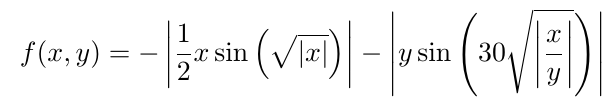
\includegraphics[width=0.5\textwidth]{images/f.PNG}
\end{figure}

This function takes 2 parameters, x and y, both these parameters will be $\in [10,1000] \cap R$.

\section{Implementation of the algorithm}
Both x and y values will be coded in binary form, and then both values will be concatenated. That is the 'genetic' code of an individual. For example, {\color{red}x = 0101010101} and {\color{blue}y = 1010101010}, this means that this individuals genetic code would be {\color{red}0101010101}{\color{blue}1010101010}.\\
There are three important steps in this algorithm, selection, crossing and mutation. Let's see how each step is done, all these steps will be done at each generation.
\subsection{Selection}
The goal is to choose the best individuals to 'live on', and the worst ones we let them 'die'. There are many ways of doing this. The way we choose to do this in this TP is the k-Tournament, this is a really easy step to selection method to understand. From the whole population at generation t, we chose 5 individuals at random (all have the same probability of being chosen), from the individuals, we keep the one with the best fitness. We do this N times, so that the number of individuals is constant through the generations.
\subsection{Crossing}
Just like in nature, we will make it so that an individual is a mix of individuals of the previous generation. This step is easily done thanks to how our individuals genetics code.\\
Lets assume we have 2 individuals:\\
\begin{center}
$individual_1$ = {\color{red}0101010101}{\color{blue}1010101010}\\
$individual_2$ = {\color{purple}1111111111}{\color{brown}0000000000}\\
\end{center}
Their corresponding children would be:
\begin{center}
$child_1$ = {\color{red}01010}{\color{purple}11111}{\color{blue}10101}{\color{brown}00000}\\
$child_2$ = {\color{purple}11111}{\color{red}10101}{\color{brown}00000}{\color{blue}01010}\\
\end{center}
However, this is only done with a given probability, $P_c$. So there is a probability $P_c$ that two individuals are crossed, and a probability $1-P_c$ that two individuals stay the same.
\subsection{Mutation}
This is the easiest step, basically for every bit in the population, there is a $P_m$ that it changes from 0 to 1, or 1 to 0. However usually this probability is very small.\\\\


\subsection{Algorithm}
\begin{itemize}
\item[(1)] Generate random population of size N
\item[(2)] For $generation\_max$ do the following steps
\item[(3)] Select Individuals, as show in section 3.1
\item[(4)] Compute crossing, as show in section 3.2 
\item[(5)] Do mutations, as show in section 3.3
\item[(6)] After doing this for $generation\_max$, return best fit individual.
\end{itemize}
\newpage
\section{Results}
The general algorithm works, but I think there might be some errors, I say this because my results aren't what I expected.\\\\
For our tests: N=100, $P_c$ = 0.6, $P_m = \{$0.1, 0.01$\}$, $max\_generation = \{$10,100,1000$\}$

\begin{center}
Mean results for 10 executions\\
\begin{tabular}{|c|cc|cc|}
\hline
{\color[HTML]{000000} max\_generation} & \multicolumn{2}{c|}{{\color[HTML]{000000} with crossing}}                                   & \multicolumn{2}{c|}{{\color[HTML]{000000} without crossing}}                                \\ \hline
{\color[HTML]{000000} -}               & \multicolumn{1}{c|}{{\color[HTML]{000000} P\_m = 0.1}} & {\color[HTML]{000000} P\_m = 0.01} & \multicolumn{1}{c|}{{\color[HTML]{000000} P\_m = 0.1}} & {\color[HTML]{000000} P\_m = 0.01} \\ \hline
{\color[HTML]{000000} 10}              & \multicolumn{1}{c|}{{\color[HTML]{000000} -1282}}      & {\color[HTML]{000000} -1275}       & \multicolumn{1}{c|}{{\color[HTML]{000000} -1283}}      & {\color[HTML]{000000} -1274}       \\ \hline
{\color[HTML]{000000} 100}             & \multicolumn{1}{c|}{{\color[HTML]{000000} -1284}}      & {\color[HTML]{000000} -1283}       & \multicolumn{1}{c|}{{\color[HTML]{000000} -1285}}      & {\color[HTML]{000000} -1285}       \\ \hline
{\color[HTML]{000000} 1000}            & \multicolumn{1}{c|}{{\color[HTML]{000000} -1284}}      & {\color[HTML]{000000} -1261}       & \multicolumn{1}{c|}{{\color[HTML]{000000} -1283}}      & {\color[HTML]{000000} -1285}       \\ \hline
\end{tabular}
\end{center}
My best result was with $max\_generation =$ 1000, $P_m =$ 0.01.\\\\
The reason why I think there are some mistakes in my code, is because the parameters don't seem to influence much the minimum.
\end{document}
